%%%%%%%%%%%%%%%%%%%%%%%%%%%%%%%%%%%%%%%%%%%%%%%%%%%%%%%%%%%%%%%%%%%%%%%%%%%%%%%%
\chapter{Proof of Concepts and Validation}\label{ch:validation}
%%%%%%%%%%%%%%%%%%%%%%%%%%%%%%%%%%%%%%%%%%%%%%%%%%%%%%%%%%%%%%%%%%%%%%%%%%%%%%%%


\section{Validation Tests}

As proof of concepts for our tool, we are going to use Mininet's emulated testbeds. We automate these tests using scripts, so they are reproducible. They are responsible for running all the proposed tests in this chapter and perform the calculations. It includes:

\begin{itemize}
	\item Build the topology;
	\item Run the SIMITAR traffic generator;
	\item Collect \textit{pcaps};
	\item Perform the proposed proof of concept analysis. 
\end{itemize}


\begin{table}[ht!]
	\centering
	\caption{Experiments specification table}
	\label{tab:specifications}
	\begin{tabular}{ll}
		\hline
		Processor            & Intel(R) Core(TM) i7-4770, 8 cores, CPU @ 3.40GHz \\
		RAM                  & 15.5 GB                                           \\
		HD                   & 1000 GB                                           \\
		Linux         & 4.8.0-59-generic                                  \\
		Ubuntu        & Ubuntu 16.10 (yakkety)                            \\
		SIMITAR       & v0.4.2 (Eulemur rubriventer)                      \\
		Mininet       & 2.3.0d1                                           \\
		Iperf         & iperf version 2.0.9 (1 June 2016) pthreads        \\
		Libtins       & 3.4-2                                             \\
		OpenDayLight  & 0.4.0-Beryllium                                   \\
		Octave        & 4.0.3                                             \\
		Pyshark       & 0.3.6.2                                     \\
		Wireshark     & 2.2.6+g32dac6a-2ubuntu0.16.10               \\
		Tcudump       & 4.9.0 \\
		libpcap       & 1.7.4\\
		\hline
	\end{tabular}
\end{table}


For each test, we generate a set of plots to compare the original and synthetic trace. Two of them we use for mere visual comparison:  flows per second and bandwidth. To compare the realism quality of the generated traffic, we plot the flows cumulative distribution function (CDF)\cite{harpoon-paper}, and the Wavelet multiresolution analysis.  In both cases, the more similar the plots are, the more similar the traffics are according to each perspective. 

The flow's cumulative distribution measures each new flow identified the trace. It is a measure similarity of the traffic at the flow-level.  The wavelet multiresolution analysis is capable of capture traffic scaling characteristics and is a measure of similarity at the packet-level. If the value decreases, a periodicity on that time scale exists. With white-noise features, the traffic will remain constant. If the traffic has self-similar characteristics on a particular time scale, its value will increase linearly.

We use two different testbeds: a tree topology (figure~\ref{fig:topo-tree}), similar to tests performed by Swing\cite{swing-paper}\cite{background-traffic-matter}\cite{legotg-paper}, and a single hop connection of two hosts. Both topologies are SDN networks and have OpenDayLight Beryllium as the controller.  We present the complete specification of these experiments at the table~\ref{tab:specifications}.
	
We generate the traffic on the host \textit{h1} with IPv4 address 10.0.0.1. The traffic is captured from the host interface with TCPdump in a \textit{pcap} format.  We organized the project directory tree as follows\footnote{ \href{https://github.com/AndersonPaschoalon/ProjetoMestrado/tree/master/Tests}{https://github.com/AndersonPaschoalon/ProjetoMestrado/tree/master/Tests} }: we placed the software at \textit{SIMITAR}. We paced the validation tests, with short tutorials at \textit{Tests} directory. The software documentation is at \textit{Docs} directory. We organized the tests as python packages, configurable by a \textit{config.py} file.


\begin{figure}[!ht]
	\centering
	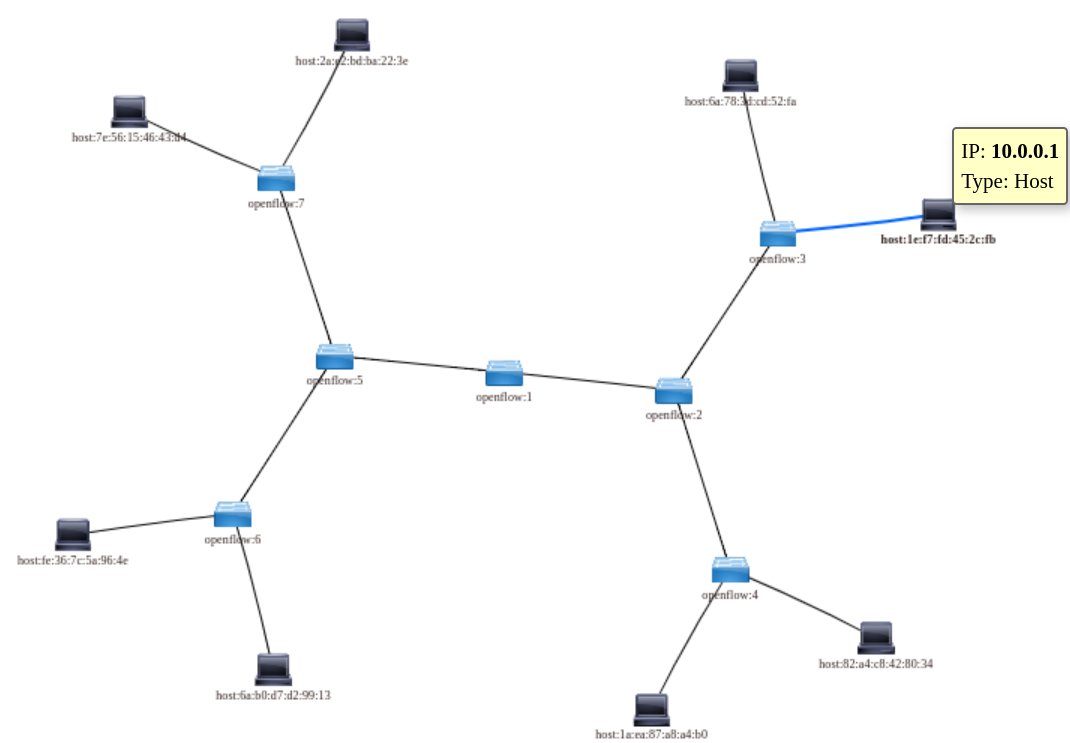
\includegraphics[scale=0.4]{figures/ch5/topo-tree}
	\caption{Tree SDN topology emulated by mininet, and controlled by OpenDayLight Beryllium}
	\label{fig:topo-tree}
\end{figure}

\begin{figure}[!ht]
	\centering
	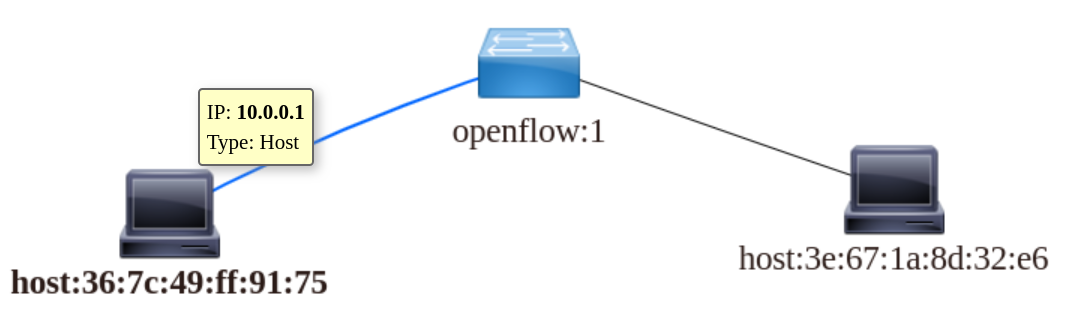
\includegraphics[scale=0.4]{figures/ch5/topo-simple}
	\caption{Single hop SDN topology emulated by mininet, and controlled by OpenDayLight Beryllium}
	\label{fig:topo-simple}
\end{figure}

We use as testbeds: a tree topology (figure~\ref{fig:topo-tree}), similar to tests performed by Swing\cite{swing-paper}\cite{background-traffic-matter}\cite{legotg-paper}, and a single hop connection of two hosts. Both topologies are SDN networks and have OpenDayLight Beryllium as the controller.  We present the complete specification of these experiments at the table~\ref{tab:specifications}.

For generating the traffic on the host \textit{h1} with IPv4 address 10.0.0.1. The traffic is captured from the host interface with TCPdump in a \textit{pcap} format.  We organized the project directory tree as follows\footnote{ \href{https://github.com/AndersonPaschoalon/ProjetoMestrado/tree/master/Tests}{https://github.com/AndersonPaschoalon/ProjetoMestrado/tree/master/Tests} }: we placed the software at \textit{SIMITAR}. We paced the validation tests, with short tutorials at \textit{Tests} directory. They are organized as python packages, and configurable by a \textit{config.py} file. The software documentation is at \textit{Docs} directory. 

We use SIMITAR v0.4.2 (Eulemur rubriventer)\footnote{ We label the tags of SIMITAR control version on GitHub as lemurs species names (\href{https://en.wikipedia.org/wiki/List_of_lemur_species}{https://en.wikipedia.org/wiki/List\_of\_lemur\_species})}, as tagged at the GitHub repository.  SIMITAR already have two functional traffic generator engines: Iperf and libtins C++ API.  

For schedule of the timing of traffic generated by each flow, we implemented three methodologies: \texttt{usleep()} C function,\texttt{select()} C function and \textit{pooling}. Here we use \texttt{usleep()} . We implemented the class \texttt{IperfFlow,} responsible for generate the traffic of each flow, using \texttt{popen()} and \texttt{pclose()} to instantiate Iperf processes, responsible for generating the traffic. Traffic customization on Iperf has many limitations. It cannot assign arbitrary IP addresses as source and destination since it must establish a connection between the source and destination. For the transport layer, it just supports TCP and UDP protocol, and constant bandwidth traffic. On the other hand, it enables customization of transmission time, number of packets, windows size, TTL, packet sizes, payload and many other features. Since Iperf has to establish a communication, SIMITAR must operate in the client mode on the source, and server mode on the destinations.

Libtins enable the creation and emission of arbitrary packets and do not require the establishment of a connection.  Thus SIMITAR does not need to operate in server mode on the destination. The packet customization capability is vast, and enable a full usage of our model parameters. Control inter-packet times stays for future work. 



\section{Results}


\begin{table}[ht!]
	\centering
	\caption{Sumary of results comparing the original traces (italic) and te traffic generated by SIMITAR, with the description of the scenario.}
	\label{my-label}
	\scalebox{0.87}{
\begin{tabular}{lcccccc}
	\hline
	\multicolumn{1}{c}{\multirow{3}{*}{}} & \multirow{3}{*}{\textit{skype-pcap}} & \multicolumn{1}{c}{\multirow{3}{*}{\begin{tabular}[c]{@{}c@{}}skype, \\ one-hop, \\ iperf\end{tabular}}} & \multicolumn{1}{c}{\multirow{3}{*}{\begin{tabular}[c]{@{}c@{}}skype, \\ tree, \\ iperf\end{tabular}}} & \multicolumn{1}{c}{\multirow{3}{*}{\begin{tabular}[c]{@{}c@{}}skype, \\ one-hop, \\ libtins\end{tabular}}} & \multirow{3}{*}{\textit{lgw10s-pcap}} & \multicolumn{1}{c}{\multirow{3}{*}{\begin{tabular}[c]{@{}c@{}}lgw10s, \\ one-hop, \\ libtins\end{tabular}}} \\
	\multicolumn{1}{c}{}                  &                             & \multicolumn{1}{c}{}                                                                                     & \multicolumn{1}{c}{}                                                                                  & \multicolumn{1}{c}{}                                                                                       &                              & \multicolumn{1}{c}{}                                                                                        \\
	\multicolumn{1}{c}{}                  &                             & \multicolumn{1}{c}{}                                                                                     & \multicolumn{1}{c}{}                                                                                  & \multicolumn{1}{c}{}                                                                                       &                              & \multicolumn{1}{c}{}                                                                                        \\ \hline
	Hurst Exponent                        & 0.601                       & 0.618                                                                                                    & 0.598                                                                                                 & 0.691                                                                                                      & 0.723                        & 0.738                                                                                                       \\
	Data bit rate (kbps)                  & 7                           & 19                                                                                                       & 19                                                                                                    & 12                                                                                                         & 7252                         & 6790                                                                                                        \\
	Average packet rate (packets/s)       & 3                           & 4                                                                                                        & 5                                                                                                     & 6                                                                                                          & 2483                         & 2440                                                                                                        \\
	Average packet size (bytes)           & 260,89                      & 549,05                                                                                                   & 481,14                                                                                                & 224,68                                                                                                     & 365,00                       & 347,85                                                                                                      \\
	Number of packets                     & 1071                        & 1428                                                                                                     & 1604                                                                                                  & 2127                                                                                                       & 24 k                         & 24 k                                                                                                        \\
	Number of flows                       & 167                         & 350                                                                                                      & 325                                                                                                   & 162                                                                                                        & 3350                         & 3264                                                                                                        \\ \hline
\end{tabular}
	}
\end{table}



% Flows per second
\begin{figure}[ht!]
	\centering
	\subfloat[\textit{Iperf, single-hop, skype-pcap}]{
		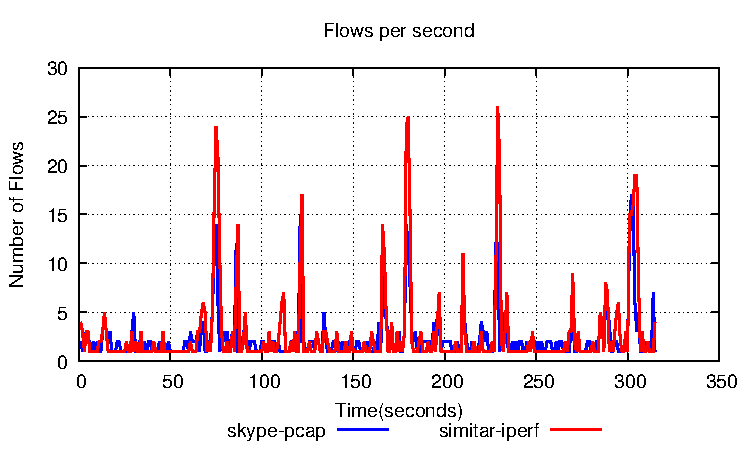
\includegraphics[width=77mm]{figures/ch5/skype-iperf-FlowsPs.pdf}
		\label{fig:iperfCdf}
	}
	\hspace{0mm}
	\subfloat[\textit{Iperf, tree, skype-pcap}]{
		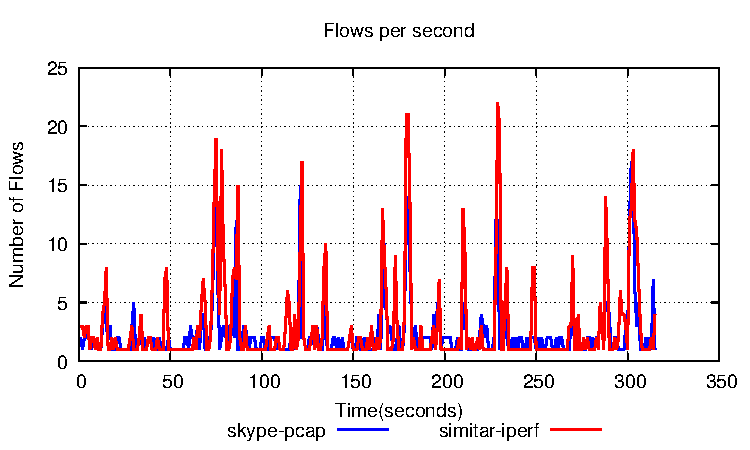
\includegraphics[width=77mm]{figures/ch5/skype-tree-iperf-FlowsPs.pdf}
		\label{fig:iperftreeCdf}
	}
	\hspace{0mm}
	\subfloat[\textit{libtins, single-hop, skype-pcap}]{
		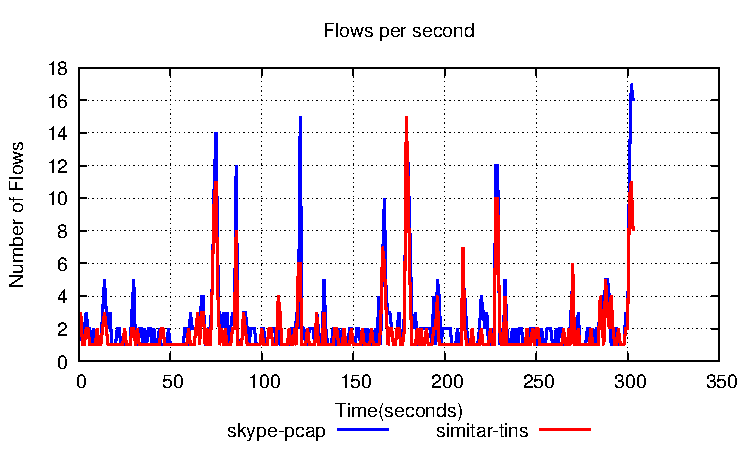
\includegraphics[width=77mm]{figures/ch5/skype-tins-FlowsPs.pdf}
		\label{fig:tinsCdf}
	}
	\hspace{0mm}
	\subfloat[\textit{libtins, single-hop, langw10s-pcap}]{
		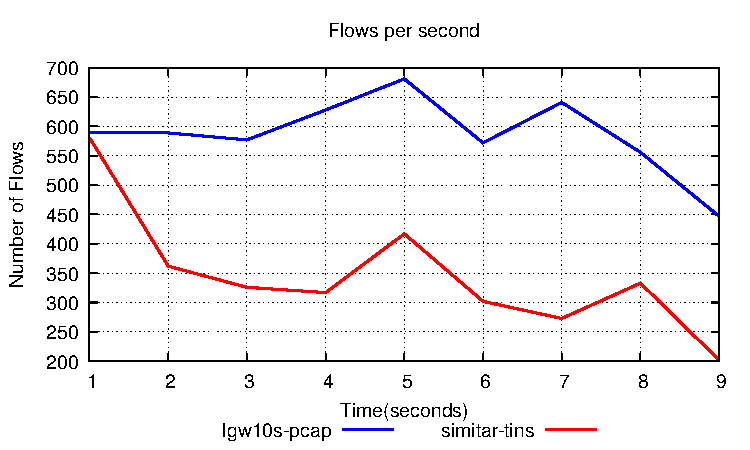
\includegraphics[width=77mm]{figures/ch5/lgw-tins-FlowsPs.pdf}
		\label{fig:tinsLgwCdf}
	}
	\hspace{0mm}
	\caption{Flow per seconds}
	\label{fig:flows-ps}
\end{figure}
% Bandwidth
\begin{figure}[h!]
	\centering
	\subfloat[\textit{Iperf, single-hop, skype-pcap}]{
		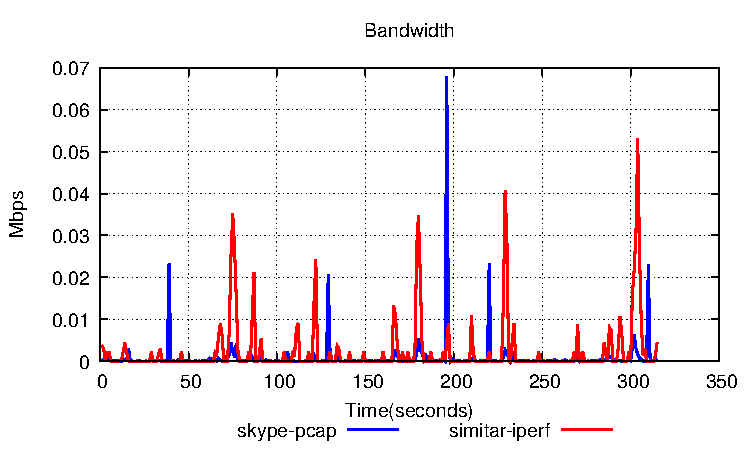
\includegraphics[width=77mm]{figures/ch5/skype-iperf-Bandwidth.pdf}
		\label{fig:iperfCdf}
	}
	\hspace{0mm}
	\subfloat[\textit{Iperf, tree, skype-pcap}]{
		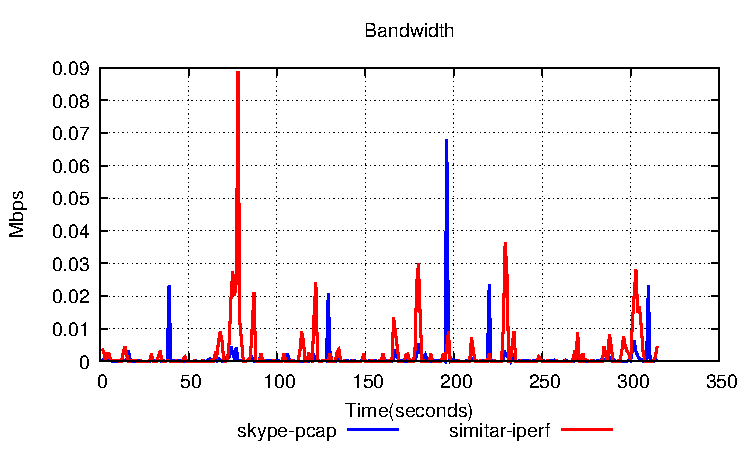
\includegraphics[width=77mm]{figures/ch5/skype-tree-iperf-Bandwidth.pdf}
		\label{fig:iperftreeCdf}
	}
	\hspace{0mm}
	\subfloat[\textit{libtins, single-hop, skype-pcap}]{
		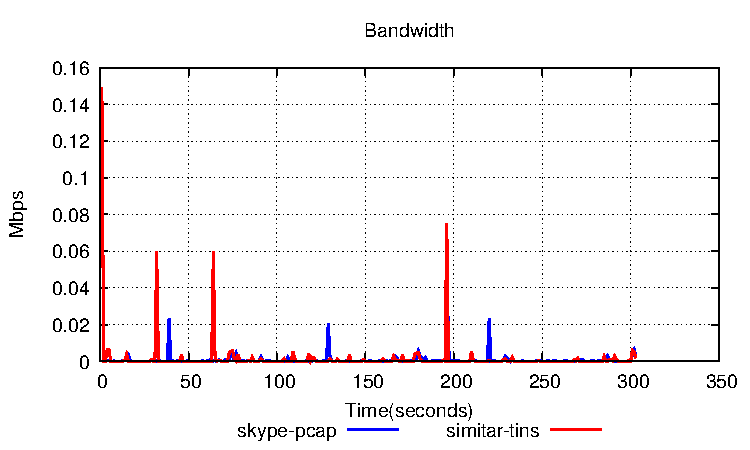
\includegraphics[width=77mm]{figures/ch5/skype-tins-Bandwidth.pdf}
		\label{fig:tinsCdf}
	}
	\hspace{0mm}
	\subfloat[\textit{libtins, single-hop, langw10s-pcap}]{
		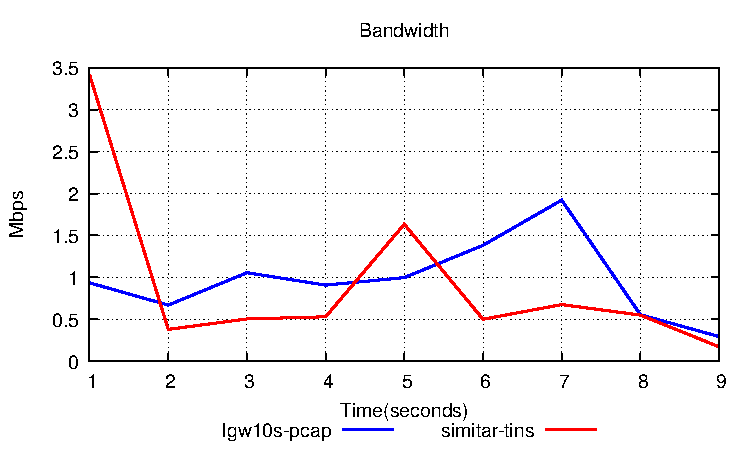
\includegraphics[width=77mm]{figures/ch5/lgw-tins-Bandwidth.pdf}
		\label{fig:tinsLgwCdf}
	}
	\hspace{0mm}
	\caption{Traces bandwidth.}
	\label{fig:flows-bandwidth}
\end{figure}
% Flow CDF
\begin{figure}[ht!]
	\centering
	\subfloat[\textit{Iperf, single-hop, skype-pcap}]{
		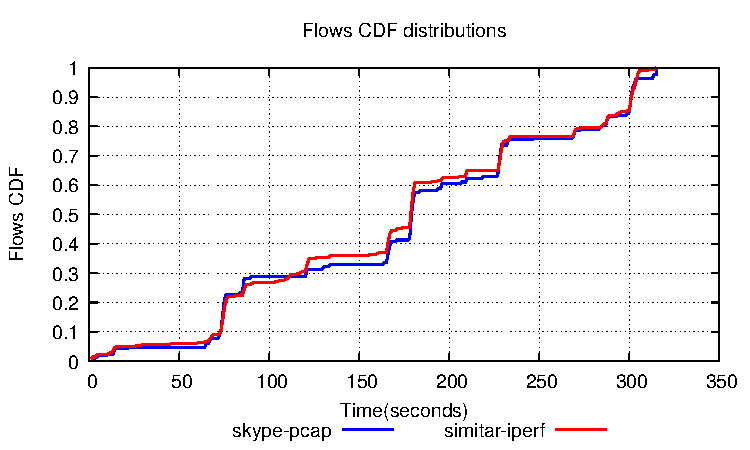
\includegraphics[width=77mm]{figures/ch5/skype-iperf-FlowCdf.pdf}
		\label{fig:iperfCdf}
	}
	\hspace{0mm}
	\subfloat[\textit{Iperf, tree, skype-pcap}]{
		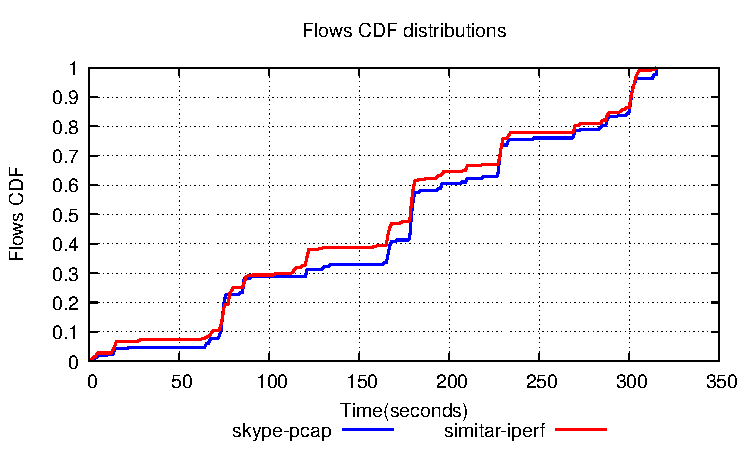
\includegraphics[width=77mm]{figures/ch5/skype-tree-iperf-FlowCdf.pdf}
		\label{fig:iperftreeCdf}
	}
	\hspace{0mm}
	\subfloat[\textit{libtins, single-hop, skype-pcap}]{
		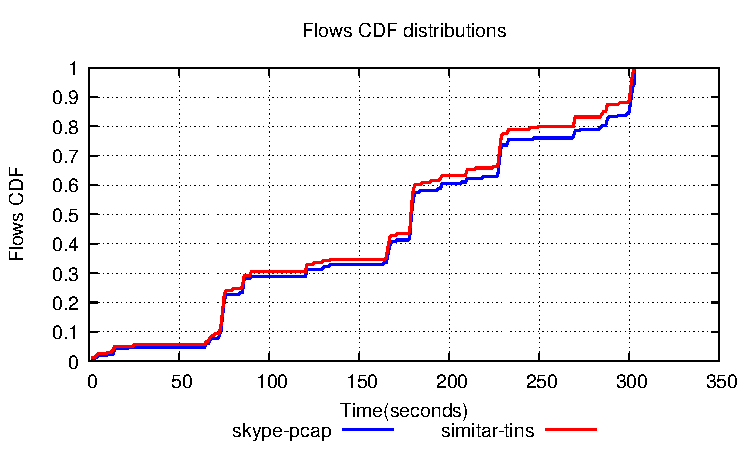
\includegraphics[width=77mm]{figures/ch5/skype-tins-FlowCdf.pdf}
		\label{fig:tinsCdf}
	}
	\hspace{0mm}
	\subfloat[\textit{libtins, single-hop, langw10s-pcap}]{
		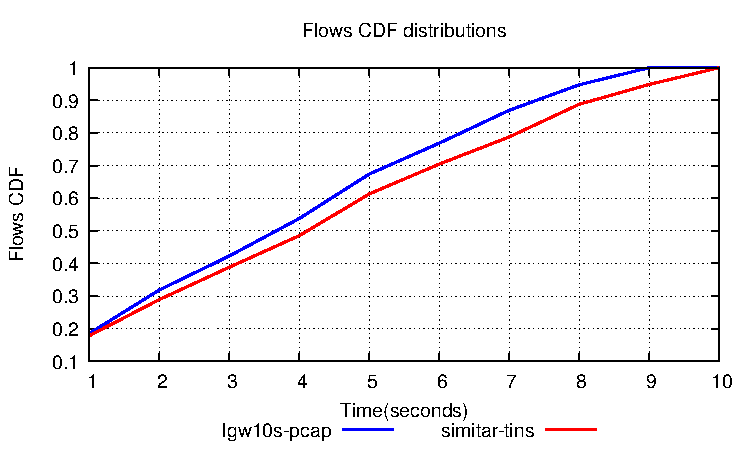
\includegraphics[width=77mm]{figures/ch5/lgw-tins-FlowCdf.pdf}
		\label{fig:tinsLgwCdf}
	}
	\hspace{0mm}
	\caption{Flows cumulative distributions.}
	\label{fig:flows-cdf}
\end{figure}
% Wabelet
\begin{figure}[h!]
	\centering
	\subfloat[\textit{Iperf, single-hop, skype-pcap}]{
		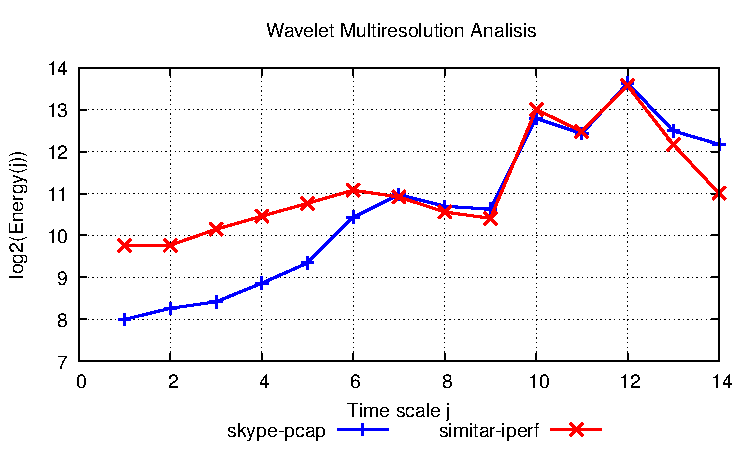
\includegraphics[width=77mm]{figures/ch5/skype-iperf-WaveletMREA.pdf}
		\label{fig:iperfWaveletMREA}
	}
	\hspace{0mm}
	\subfloat[\textit{Iperf, tree, skype-pcap}]{
		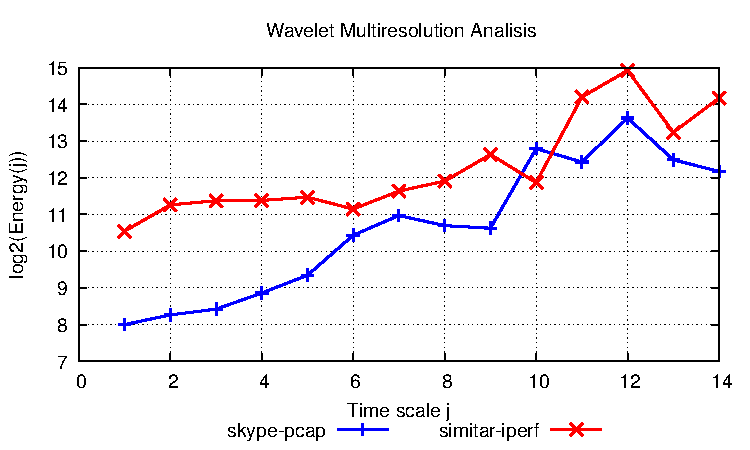
\includegraphics[width=77mm]{figures/ch5/skype-tree-iperf-WaveletMREA.pdf}
		\label{fig:iperftreeWaveletMREA}
	}
	\hspace{0mm}
	\subfloat[\textit{libtins, single-hop, skype-pcap}]{
		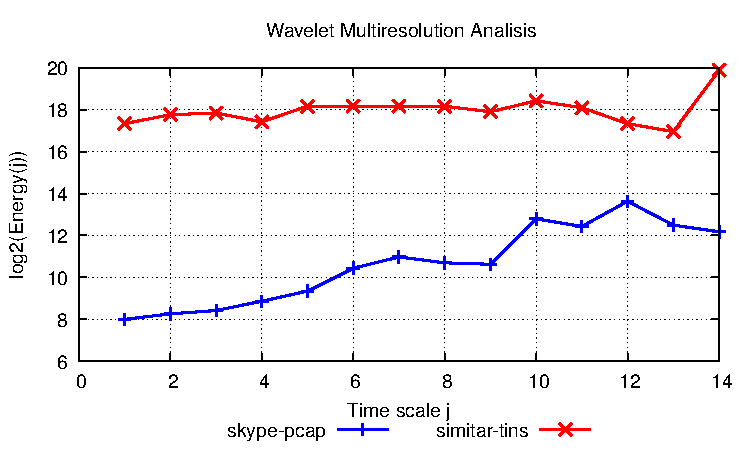
\includegraphics[width=77mm]{figures/ch5/skype-tins-WaveletMREA.pdf}
		\label{fig:tinsWaveletMREA}
	}
	\hspace{0mm}
		\subfloat[\textit{libtins, single-hop, langw10s-pcap}]{
			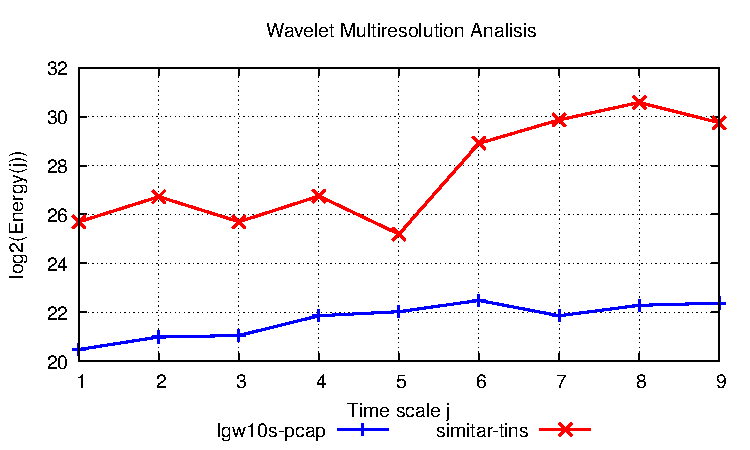
\includegraphics[width=77mm]{figures/ch5/lgw-tins-WaveletMREA.pdf}
			\label{fig:tinsLgwWaveletMREA}
		}
		\hspace{0mm}
	\caption{Wavelet multiresolution energy analysis.}
	\label{fig:wavelet}
\end{figure}





\section{Current Limitations}



To evaluate the Scalling profile of the traccic generator, we are usig the same validation used for Swing\cite{swing-paper}: multiresolution energy analysis.
